%%%%%%%%%%%%%%%%%%%%%%%%%%%%%%%%%%%%%%%%
\chapter{Introduzione}
\label{cap1}
%%%%%%%%%%%%%%%%%%%%%%%%%%%%%%%%%%%%%%%%
%cap1-ICNSC-2017.pdf
%http://ieeexplore.ieee.org/document/8000145/

Questa sarà un era in cui gli utenti interagiranno con un ambiente digitale ed intelligente \cite{Fortino2014}, piena di opportunità \cite{GUBBI20131645} che cambierà significativamente il modo di vivere l'ambiente e la tecnologia; uno dei paradigmi computazionali emergenti è l’Internet of Things (IoT, Internet Delle Cose). Basato sulla collaborazione tra oggetti virtuali e fisici \cite{fortino2014internet}, \cite{fortino2014integration}. 
E' costituito da sensori, ognuno con differenti caratteristiche, in grado di interagire con l’ambiente circostante e con capacità di comunicazione che permettono di supportare l’utente tramite servizi eterogenei \cite{8000145}.
\begin{figure}[h]
	\centering
	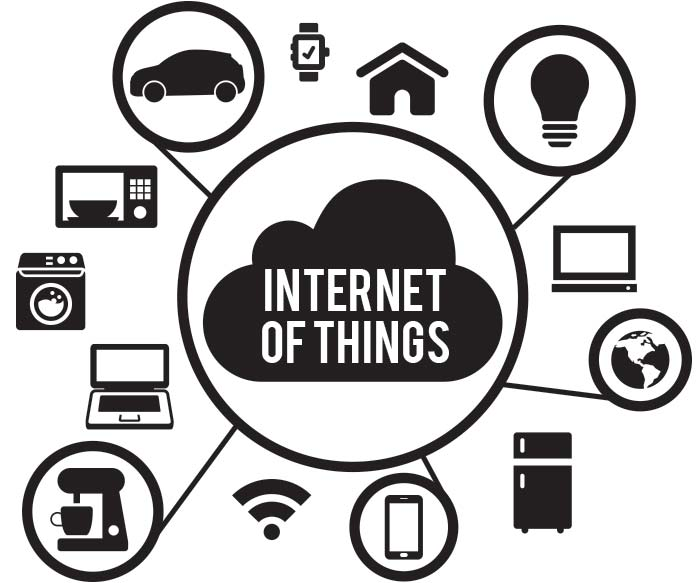
\includegraphics[width=0.7\linewidth]{imgs/Internet-of-Things-IoTgraphic}
	\caption[Internet Of Things]{Internet Of Things}
	\label{fig:internet-of-things-iotgraphic}
	%https://thenewstack.io/what-does-it-mean-to-be-on-the-internet-of-things/
\end{figure}

Quando si parla di ambienti intelligenti si indicano varie entità tra cui:
\begin{itemize}
	\item Smart Home (case intelligenti)
	\item Smart City (città intelligenti)
	\item Smart Transportation (trasporti intelligenti)
	\item Smart Office (uffici intelligenti)
	\item etc.
\end{itemize}
%cap1-SmartEducation-2017.pdf
%http://ieeexplore.ieee.org/document/7962537/

Ognuno di questi ambienti intelligenti, con cui l'utente interagisce, sarà dotato di oggetti (Things, Cose) intelligenti, dispositivi elettronici, sempre più piccoli, anche alimentati a batteria con l'ausilio di radio trasmettitori e microcontrollori che, come predetto dalla legge di Moore, hanno consumo energetico decrescente così come le loro dimensioni.

Tramite questi dispositivi si può realizzare l’IoT poiché ognuno di essi è capace di interagire con l’ambiente circostante rimanendo collegato ad internet \cite{ashton2009internet} \cite{swan2012sensor}, si può vedere una rappresentazione visiva del concetto IoT\textbf { illustrata in figura} \ref{fig:internet-of-things-iotgraphic}. %SINTEF+S13363.pdf 
Una “Cosa” quindi è un’entità che esiste e si muove nel tempo e nello spazio, può essere reale o virtuale ma deve avere un'identità nella rete stabilita tramite ID, indirizzi o nomi\cite{SINTEF+S13363}. %cap1- iot.pdf
Questo varrà dire che, sotto diversa forma, molti degli oggetti che ci circondano saranno nella rete \cite{gubbi2013internet}.

%Cap1-IMPORTANTE-morin2017.pdf
L’obiettivo dell’IoT quindi è quello di utilizzare il protocollo IP per connettere ad internet questi dispositivi, permettendo lo sviluppo di nuove applicazioni per la comunicazione. Alcune delle problematiche legate a questi dispositivi riguardano il consumo energetico, poiché l’idea è quella di avere dispositivi a batteria con un tempo-vita di diversi anni prima che sia sostituita. Ancor più impegnative sono le operazioni a basso consumo per quei dispositivi che acquisiscono energia dall’ambiente, ad esempio con dei pannelli solari, poiché dovranno essere compensati i momenti di utilizzo dell’energia con una successiva assunzione di energia\cite{morin2017comparison}.
%\begin{figure}
	%cap1-gs-1402.4675.pdf
%	\centering
%	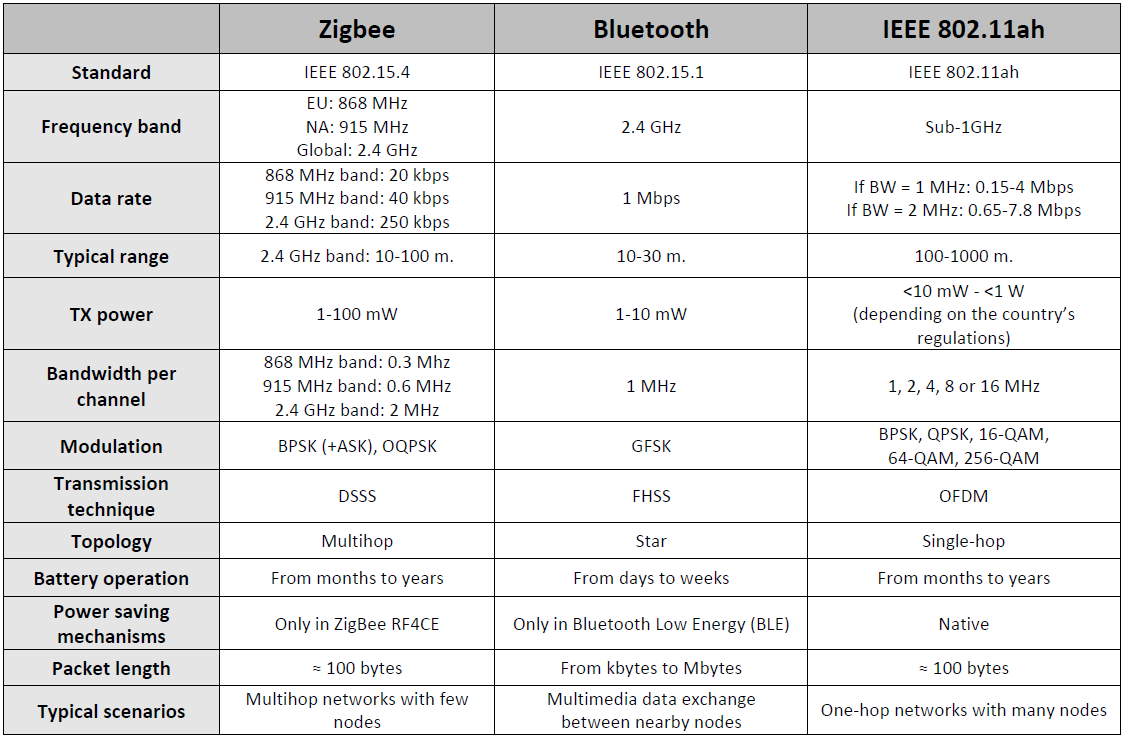
\includegraphics[width=1\linewidth]{imgs/1-confrontoZigbeeBluetoothHaLow.png}
%	\caption[Tavole Comparative]{Tavole Comparative \cite{7000982}}
%	\label{fig:1-confronto}
%\end{figure}

%Cap1-IMPORTANTE-morin2017.pdf
Lo standard 802.15.4 è stato recentemente utilizzato per realizzare dispositivi a bassa potenza\cite{ieee2003ieee} essendo progettato appositamente per un basso consumo energetico. Tozlu, tramite la sua ricerca\cite{5982548}, ha potuto evidenziare che anche i dispositivi 802.11 con standard 802.11b godono di una buona efficienza energetica grazie al Power Saving Mode(PSM)\cite{ieee1999part11} tanto da superare quella dell’802.15.4. Un'altra soluzione a corto raggio con basso consumo energetico, è il Bluetooth Low Energy (BLE) \cite{Bluetooth502016}, ma emergono soluzioni a lungo raggio come 802.11ah \cite{7558107} oppure LoRa \cite{LoRa2017} e SIGFOX \cite{SIGFOX2017} che competono nel mercato LPWAN (Low-Power Wide-Area Network). Nella panoramica comparativa \textbf {nelle figure} \ref{fig:0-confronto} \ref{fig:01-confronto} si possono osservare svariati standard IoT messi a confronto, ognuno di essi ha delle specifiche che possono essere attrattive per casi di utilizzo differenti nell'ambito IoT

\begin{figure}
	\centering
	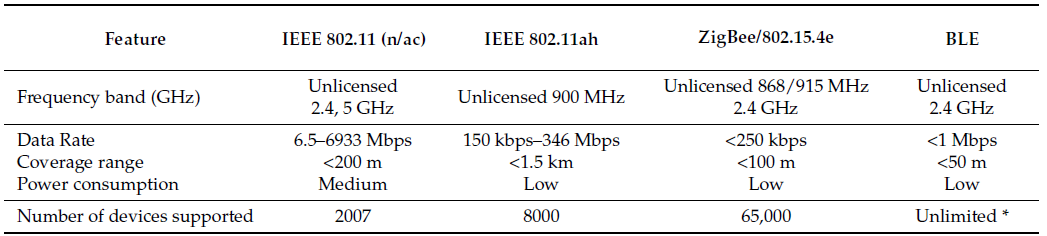
\includegraphics[width=1\linewidth]{imgs/0-confronto}
	\caption[Confronto standard]{Panoramica confronto standard IoT \cite{banos2016ieee}}
	\label{fig:0-confronto}
\end{figure}

\begin{figure}
	\centering
	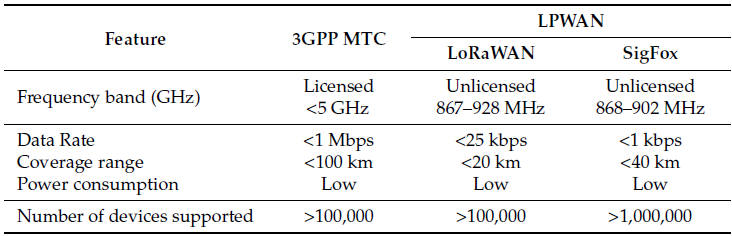
\includegraphics[width=0.7\linewidth]{imgs/01-confronto}
	\caption[Confronto standard]{Panoramica confronto standard IoT \cite{banos2016ieee}}
	\label{fig:01-confronto}
\end{figure}



%cap1-IMPORTANTE-sensors-16-01960.pdf
Nel mercato IoT lo standard IEEE 802.11, originariamente sviluppato per scenari domestici ed uffici, non mostrava alcuna presenza significativa ma è ampiamente utilizzato in una vasta gamma di dispositivi elettronici di consumo e in diversi scenari. Considerando che lo scenario delle comunicazioni IoT è sempre più prossimo la Wi-Fi Alliance ha deciso di colmare la mancanza introducendo il nuovo standard 802.11ah ed il "Wi-Fi HaLow Program" basto sul nuovo standard di cui si attende la certificazione ed il lancio nel 2018. Tramite questo standard le funzionalità specifiche dell’IoT potranno essere abilitate in migliaia di stazioni che operano a frequenze sotto 1Ghz (ISM, Industrial, Scientific and Medical)\cite{7000982}\cite{7101216}\cite{sun2013ieee}.
E' stato designato per \cite{banos2016ieee}:

\begin{itemize}
	\item Smart sensors and meters (Sensori e misuratori intelligenti); l'obbiettivo è quello di avere una copertura per le applicazioni IoT sia in ambienti interni che esterni; 
	\item Backhaul aggregation (globalizzazione del carico di ritorno);questo scenario prevede che i dati acquisiti dai dispositivi (i.e., sensori) siano raccolti da routers o gateways ed inoltrati ai servers; 
	\item Extended range hotspot and cellular offloading (Hotspot a lungo raggio e riduzione del traffico); sia la trasmissione a lungo raggio che l'alto rendimento di questo protocollo sono molto attraenti per migliorare l'hotspot o per permettere una riduzione di carico per il traffico nelle reti mobili;
	\item Ed altri casi d'uso per future applicazioni che lo IEEE 802.11 WG(Working Group) ha innescato tramite la realizzazione di svariati WG differenti che operano su diversi fronti. 
\end{itemize}


Come evidenziato in \textbf {figura} \ref{fig:0-confronto} lo standard IEEE 802.11ah gode di un ottima adattabilità sia ad utilizzi a corto che lungo raggio avendo una copertura che può arrivare fino ad 1.5 Km.

L'obbiettivo di questo elaborato è quello di analizzare lo standard 802.11ah sia nei dettagli del protocollo sia nei casi d'uso dello stesso in ambito IoT, spiegando come questo protocollo può soddisfare le richieste delle applicazioni IoT:
\begin{itemize}
	\item nel Secondo capitolo verrà analizzato lo standard 802.11ah nel dettaglio di quello che è il livello fisico e il livello MAC, porgendo particolare attenzione ai meccanismi di risparmio energetico ed evidenziando le differenze tra questo e le altre versioni 802.11
	\item nel Terzo capitolo verranno analizzati alcuni scenari in ambito IoT e verrà posta a particolare attenzione ad alcuni di questi che potrebbero essere ben supportati dallo standard 802.11ah 
	\item nel Quarto capitolo verranno posti i risultati degli approcci analizzati.
	\item capitolo 5 conclusioni
\end{itemize}
    

%cap1-IMPORTANTE-sensors-16-01960.pdf



%%%%%%%%%%%%%%%%%%%%%%%%%%%%%%%%%%%%%%%%
\clearpage